% !TeX program = pdflatex
\documentclass[tikz,border=8pt]{standalone}
\usepackage{pgfplots}
\pgfplotsset{compat=1.16}
\definecolor{FigureBlue}{HTML}{2563EB}
\definecolor{FigureOrange}{HTML}{EA580C}
\definecolor{FigureGreen}{HTML}{16A34A}
\definecolor{FigurePurple}{HTML}{7C3AED}
\definecolor{FigureSlate}{HTML}{475569}
\begin{document}
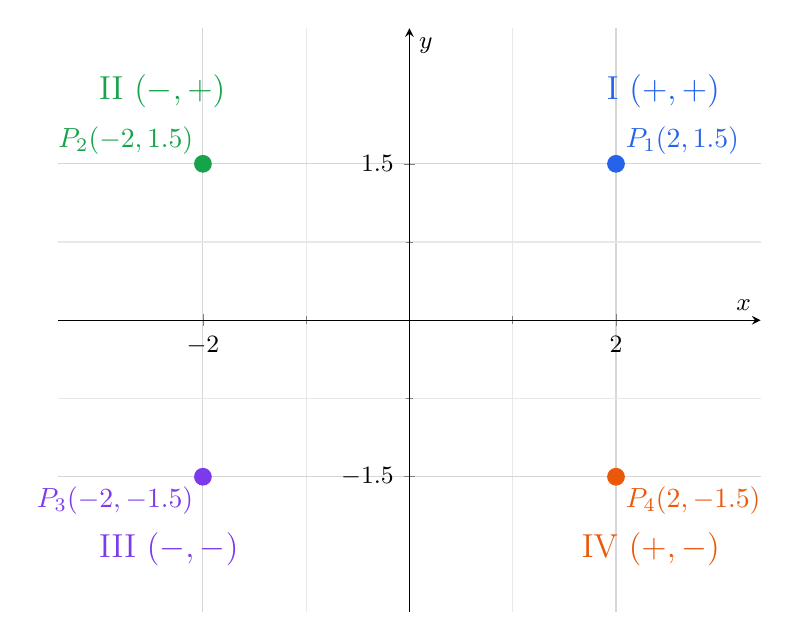
\begin{tikzpicture}
  \begin{axis}[
    width=10.5cm,height=9cm,
    axis lines=middle,
    xmin=-3.4,xmax=3.4,ymin=-2.8,ymax=2.8,
    xlabel={$x$},ylabel={$y$},
    xtick={-2,0,2},ytick={-1.5,0,1.5},
    grid=both,minor tick num=1,
    grid style={draw=gray!18},major grid style={draw=gray!32},
    tick label style={font=\small},label style={font=\small},
    clip=false,
  ]
    \addplot[only marks,mark=*,mark size=3pt,FigureBlue] coordinates {(2,1.5)};
    \addplot[only marks,mark=*,mark size=3pt,FigureGreen] coordinates {(-2,1.5)};
    \addplot[only marks,mark=*,mark size=3pt,FigurePurple] coordinates {(-2,-1.5)};
    \addplot[only marks,mark=*,mark size=3pt,FigureOrange] coordinates {(2,-1.5)};
    \node[anchor=south west,text=FigureBlue] at (axis cs:2,1.5) {$P_1(2,1.5)$};
    \node[anchor=south east,text=FigureGreen] at (axis cs:-2,1.5) {$P_2(-2,1.5)$};
    \node[anchor=north east,text=FigurePurple] at (axis cs:-2,-1.5) {$P_3(-2,-1.5)$};
    \node[anchor=north west,text=FigureOrange] at (axis cs:2,-1.5) {$P_4(2,-1.5)$};
    \node[anchor=north east,text=FigureBlue,font=\large] at (axis cs:3.1,2.45) {I $(+,+)$};
    \node[anchor=north west,text=FigureGreen,font=\large] at (axis cs:-3.1,2.45) {II $(-,+)$};
    \node[anchor=south west,text=FigurePurple,font=\large] at (axis cs:-3.1,-2.45) {III $(-,-)$};
    \node[anchor=south east,text=FigureOrange,font=\large] at (axis cs:3.1,-2.45) {IV $(+,-)$};
  \end{axis}
\end{tikzpicture}
\end{document}
